\documentclass[]{article}
\usepackage[T1]{fontenc}
\usepackage{lmodern}
\usepackage{amssymb,amsmath}
\usepackage{ifxetex,ifluatex}
\usepackage{fixltx2e} % provides \textsubscript
% use upquote if available, for straight quotes in verbatim environments
\IfFileExists{upquote.sty}{\usepackage{upquote}}{}
\ifnum 0\ifxetex 1\fi\ifluatex 1\fi=0 % if pdftex
  \usepackage[utf8]{inputenc}
\else % if luatex or xelatex
  \ifxetex
    \usepackage{mathspec}
    \usepackage{xltxtra,xunicode}
  \else
    \usepackage{fontspec}
  \fi
  \defaultfontfeatures{Mapping=tex-text,Scale=MatchLowercase}
  \newcommand{\euro}{€}
\fi
% use microtype if available
\IfFileExists{microtype.sty}{\usepackage{microtype}}{}
\usepackage{graphicx}
% Redefine \includegraphics so that, unless explicit options are
% given, the image width will not exceed the width of the page.
% Images get their normal width if they fit onto the page, but
% are scaled down if they would overflow the margins.
\makeatletter
\def\ScaleIfNeeded{%
  \ifdim\Gin@nat@width>\linewidth
    \linewidth
  \else
    \Gin@nat@width
  \fi
}
\makeatother
\let\Oldincludegraphics\includegraphics
{%
 \catcode`\@=11\relax%
 \gdef\includegraphics{\@ifnextchar[{\Oldincludegraphics}{\Oldincludegraphics[width=\ScaleIfNeeded]}}%
}%
\ifxetex
  \usepackage[setpagesize=false, % page size defined by xetex
              unicode=false, % unicode breaks when used with xetex
              xetex]{hyperref}
\else
  \usepackage[unicode=true]{hyperref}
\fi
\hypersetup{breaklinks=true,
            bookmarks=true,
            pdfauthor={CS544 — MP 1},
            pdftitle={Abdul Dakkak},
            colorlinks=true,
            citecolor=blue,
            urlcolor=blue,
            linkcolor=magenta,
            pdfborder={0 0 0}}
\urlstyle{same}  % don't use monospace font for urls
\setlength{\parindent}{0pt}
\setlength{\parskip}{6pt plus 2pt minus 1pt}
\setlength{\emergencystretch}{3em}  % prevent overfull lines
\setcounter{secnumdepth}{0}

\title{Abdul Dakkak}
\author{CS544 --- MP 1}
\date{}

\begin{document}
\maketitle

\begin{quote}
My research area is compilers and architecture. Attempts were made to
apply optimization to my area, but they were abandoned since they were
quite a bit involved for a homework project. It is my hope to use
optimization for instruction selection (in the compiler) for my class
project.
\end{quote}

In this report we will examine the differences of Quasi-Newton's method
and Polak Ribiere using 2 criterions. We will then look at how efficient
it is at finding the solution. To facilitate this, we will be finding
the minimum for a function of two variables. The final criteria is how
well it performs in practice for a sample application. We will use
Poisson blending of two images here.

\subsection{Exploration in 2D}\label{exploration-in-2d}

We start by exploring the two methods using functions of 2 arguments.
The figure bellow shows the results. As can be observed, Newton's method
takes more steps but evaluates the function a few times less. Polak
Ribier take less steps and evaluates the equation more times.

\begin{figure}[t!]
\centering
\includegraphics[scale=0.05]{exp.png}
\caption{Experimentation between Quasi-Newton and Polak Ribiere. The first column shows the function to be minimized, the second show the Quasi-Newton results, and the third show the results from Polak Ribiere.}
\label{fig:exp}
\end{figure}

Figuring out which one to choose in this case would be dependent on how
complicated the function is. If evaluation of the function would take a
long time, then PR would be used and Newton would be used otherwise.

\subsection{Poisson Blending}\label{poisson-blending}

To evaluate the methods using thousands of variables, we will use posson
blending (as said previously it took quite a bit of time to find an
application outside my field that was still interesting : other
applications examined were neural networks, image segementation using
mean shift, and genetic algorithms).

Given two images source $S$ and target $T$ with an acomaning mast $M$.
The Poisson blending method performs a cut and paste image operation
from $S$ to $T$ minimizing the variation at the boundary.
Mathematically, we want to minimize the variation within the mask within
the contraint that the boundary values must come from the target image.

\[
\underset{f}{\text{min}} \iint \limits_\Omega \|  f \|
\]

with $f^* \lvert_{\partial \Omega} = f \lvert_{ \partial \Omega}$

This is a least squares minimization problem that can be solved by
constructing the equation $Ax = b$ and solving for $x$. Where $x$ is an
$N \times N$ vector corresponding to the output pixels, and $A$ is an
$(N \times N) \times (N \times N)$ matrix corresponding to the
constraints, and $b$ corresponds to the known values. The matrix $A$ is
constructed by

\begin{verbatim}
for ii from 0 to N:
    for jj from 0 to N:
        A[idx(ii, jj), idx(ii, jj)] = -4
        B[idx(ii, jj)] = 4*S[ii, jj] - S[ii + 1, jj + 1] -
                           S[ii + 1, jj - 1] - S[ii - 1, jj + 1] +
                           S[ii - 1, jj - 1]
        for (x,y) in [(1, 1), (-1, -1), (1, -1), (-1, 1)] :
            if M[ii + x, jj + y] == 0
                A[idx(ii, jj), idx(ii + x, jj + y)] = -1
            else
                B[idx(ii + y, jj + x)] -= T[ii + x,jj + y]
\end{verbatim}

with \texttt{idx} being an auxilary function defined by

\begin{verbatim}
idx(ii, jj) := ii*(N*N) + jj
\end{verbatim}

It is clear that $A$ is a very sparse matrix with at most $4$ entries in
each row.

\subsubsection{Poisson Blending Results}\label{poisson-blending-results}

We now evaluate solving for $x$ using both Quasi-Newton and Polak
Ribiere based least squares solver. We will varry the number of unknown
by resizing the input images.

\begin{figure}[htbp]
\centering
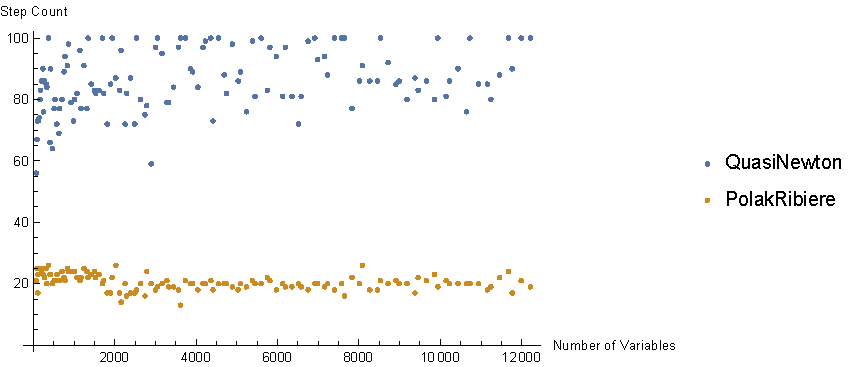
\includegraphics{step.pdf}
\caption{The number of steps taken to solve the linear squares problem
as we vary the number of variables being solved.}
\end{figure}

\begin{figure}[t!]
\centering
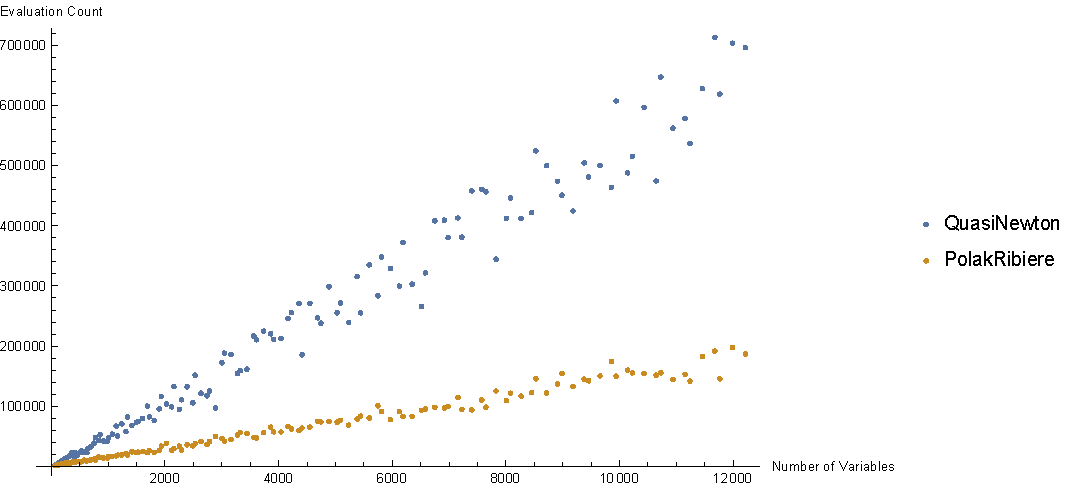
\includegraphics{eval.pdf}
\caption{The number of times the function has been evaluated as we vary the number of variables being solved.}
\label{fig:eval}
\end{figure}

The previous two measures contribute the effective execusion time of the
algorithm. Figure \ref{fig:time} shows the execution times in seconds.
As can be seen, Polak Ribiere is around 2 to 2.5 times faster than
Quasi-Newton.

\begin{figure}[t!]
\centering
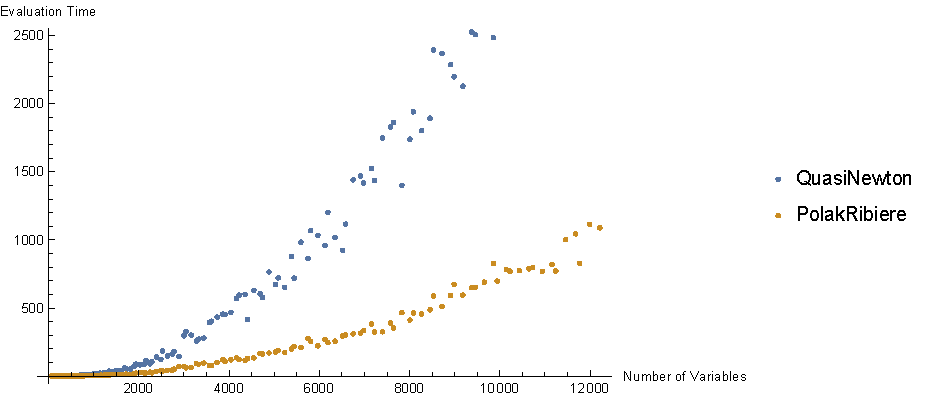
\includegraphics{time.pdf}
\caption{The time to solve the linear squares problem as we vary the number of variables being solved.}
\label{fig:time}
\end{figure}

\subsection{Conclusion}\label{conclusion}

Based on the experiments, Polak Ribiere outperfromed Quasi-Newton in the
evaluation time, step count, and evaluation count metrics. We expect
that Quasi-Newton to take less memory than Polak Ribiere, but that has
not been measured. So, to answer the original question, I would choose
Polak Ribiere as my go-to method to solve linear least squares.

\end{document}
